\chapter{\texorpdfstring{Evaluation of the corrected \ds/\dpl yield ratio}{Evaluation of the corrected Ds+/D+ yield ratio}}\label{ch:corrections}

To evaluate the ratio between the production yield ratio of the two D-meson species, a number of corrections must be applied to the extracted raw yields. These corrections are necessary to account for the acceptance of the detector, the selection efficiency of \ds and \dpl mesons, the branching ratio of the decay channels, and the feed-down from beauty-hadron decays. The prompt \ds/\dpl production yield ratio is then obtained by dividing the corrected yield of \ds mesons by the corrected yield of \dpl mesons:
\begin{equation}\label{eq:DsDplusRatio}
        \ds/\dpl = \frac{N_\mathrm{raw}^{\ds}\cdot \fpds}{\aeffpds \cdot \mathrm{BR}^\ds} \cdot \left(\frac{N_\mathrm{raw}^{\dpl}\cdot \fpdpl}{\aeffpdpl \cdot \mathrm{BR}^\dpl}\right)^{-1}\quad ,
\end{equation}
where \aeffp is the product of the detector acceptance and the efficiency of the selections for promptly-produced D mesons, \fp is the fraction of prompt D mesons in the extracted raw yield, and BR is the branching ratio of the considered decay channel. 

In the following sections, a detailed description of the corrections applied to the raw yields is given.

\section{Acceptance and efficiency correction}\label{sec:aeff}
The first correction takes into account that only a fraction Acc (the detector's \emph{acceptance}) of the produced D mesons can be detected by the ALICE apparatus, due to the geometry of the detector. As the tracks are reconstructed in the pseudorapidity region $\lvert\eta\rvert<0.8$, the acceptance is limited to $\lvert y\rvert<0.8$ at high \pt ($\gtrsim5~\gevc$) and to $\lvert y\rvert<0.5$ for $\pt\sim0$, as shown in Fig.~\ref{fig:RapidityAcceptance}. Due to the very similar decay topology and kinematics of the \ds and \dpl mesons in the considered decay channel, this term is expected to cancel out in the ratio of the two species' production yields. Additionally, only a fraction $\varepsilon$ (the reconstruction and selection \emph{efficiency}) of the detectable D mesons passes the selection criteria described in Chapters~\ref{chap:reconstruction} and \ref{chap:RY}. The efficiency term $\varepsilon$ also includes the reconstruction efficiency of the D meson daughter particles.

These corrections are evaluated using a sample of \ds and \dpl mesons from Monte Carlo (MC) simulations. To avoid the introduction of biases, a different data sample is used for the evaluation of the acceptance and efficiency corrections compared to the one used for the ML model training and performance evaluation. Proton-proton collisions are simulated using the \textsc{Pythia~8} event generator~\cite{Bierlich:2022pfr} with colour-reconnection Mode~2~\cite{Christiansen:2015yqa}. As for the MC simulations employed for the ML training, the MC dataset is enriched of heavy-flavour hadrons by only selecting events where at least a $\mathrm{c\overline{c}}$ or $\mathrm{b\overline{b}}$ pair is produced. The generated particles are propagated through the ALICE experimental apparatus using the \textsc{Geant4} transport simulation toolkit~\cite{GEANT4:2002zbu}. Due to the displaced topology of heavy-flavour decays and the continuous readout employed by the ALICE detector, events with charm or beauty hadrons are frequently affected by ``fake'' primary vertices arising from the association of displaced decay tracks, thereby degrading the reconstruction of heavy-flavour hadrons. The inefficiency in the reconstruction due to the presence of many heavy-flavour hadrons in nearby events is worse in MC simulations than in data, as heavy-flavour hadrons are produced more frequently than in data and the time resolution on the tracks does not always allow for their non-ambiguous association to a single collision. To overcome this problem, minimum bias events are generated between charm- or beauty-triggered ones (\emph{gap-triggered} approach). Studies performed using different gap sizes have shown that a gap of 4 minimum bias events between heavy-flavour-triggered events reduces the number of fake vertices to an acceptable level, while keeping the simulation time reasonable.

\begin{figure}[tb]
    \begin{center}
    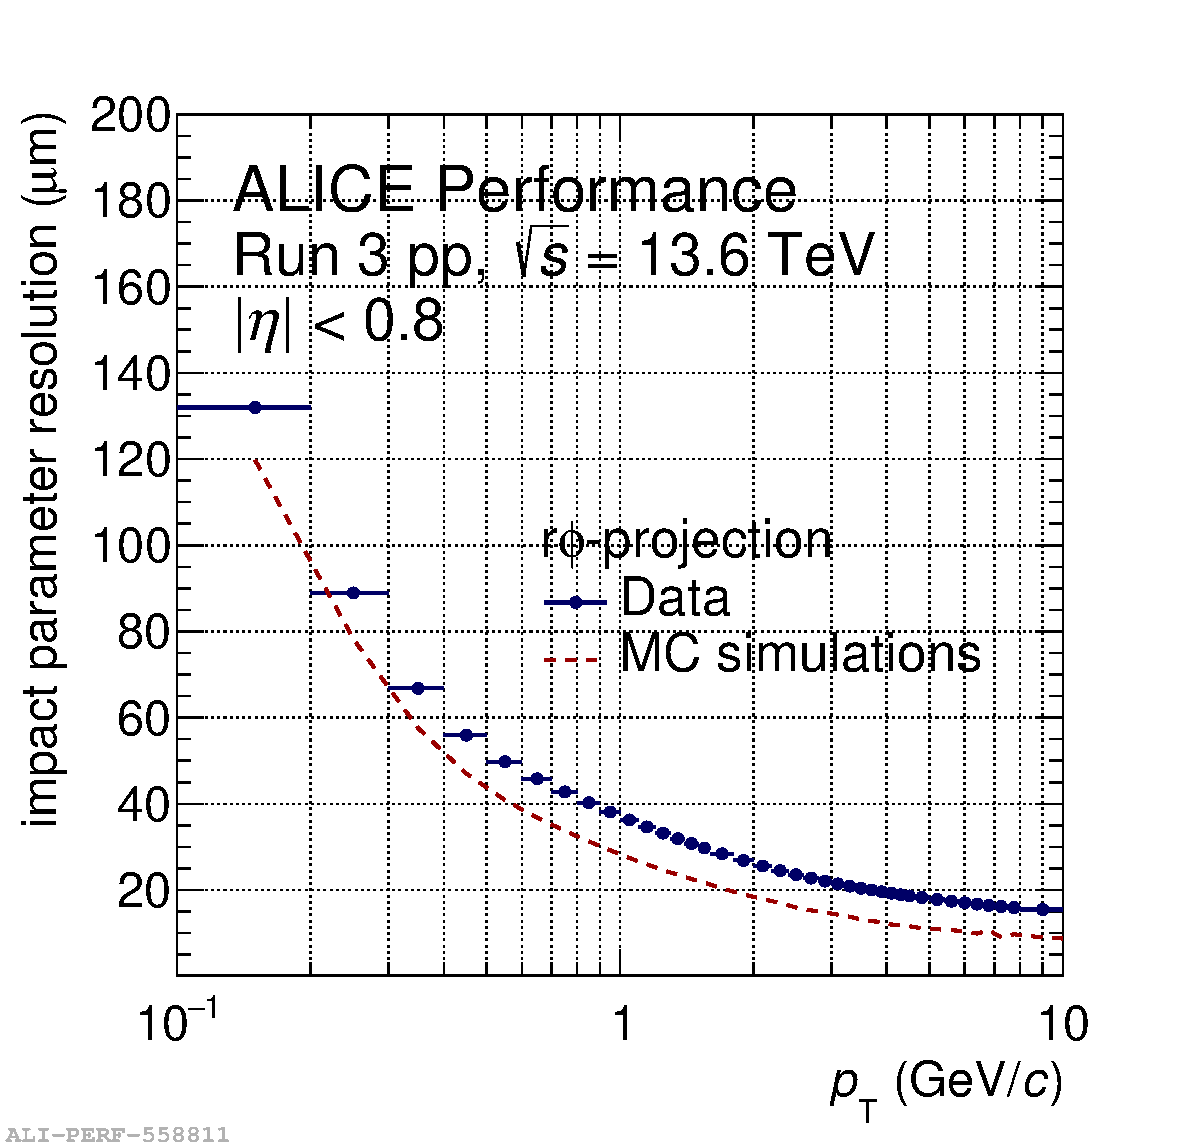
\includegraphics[width=0.48\textwidth]{Figures/Chapter 6/sigmadcaxy_lhc22o_pass4_qm.pdf}
    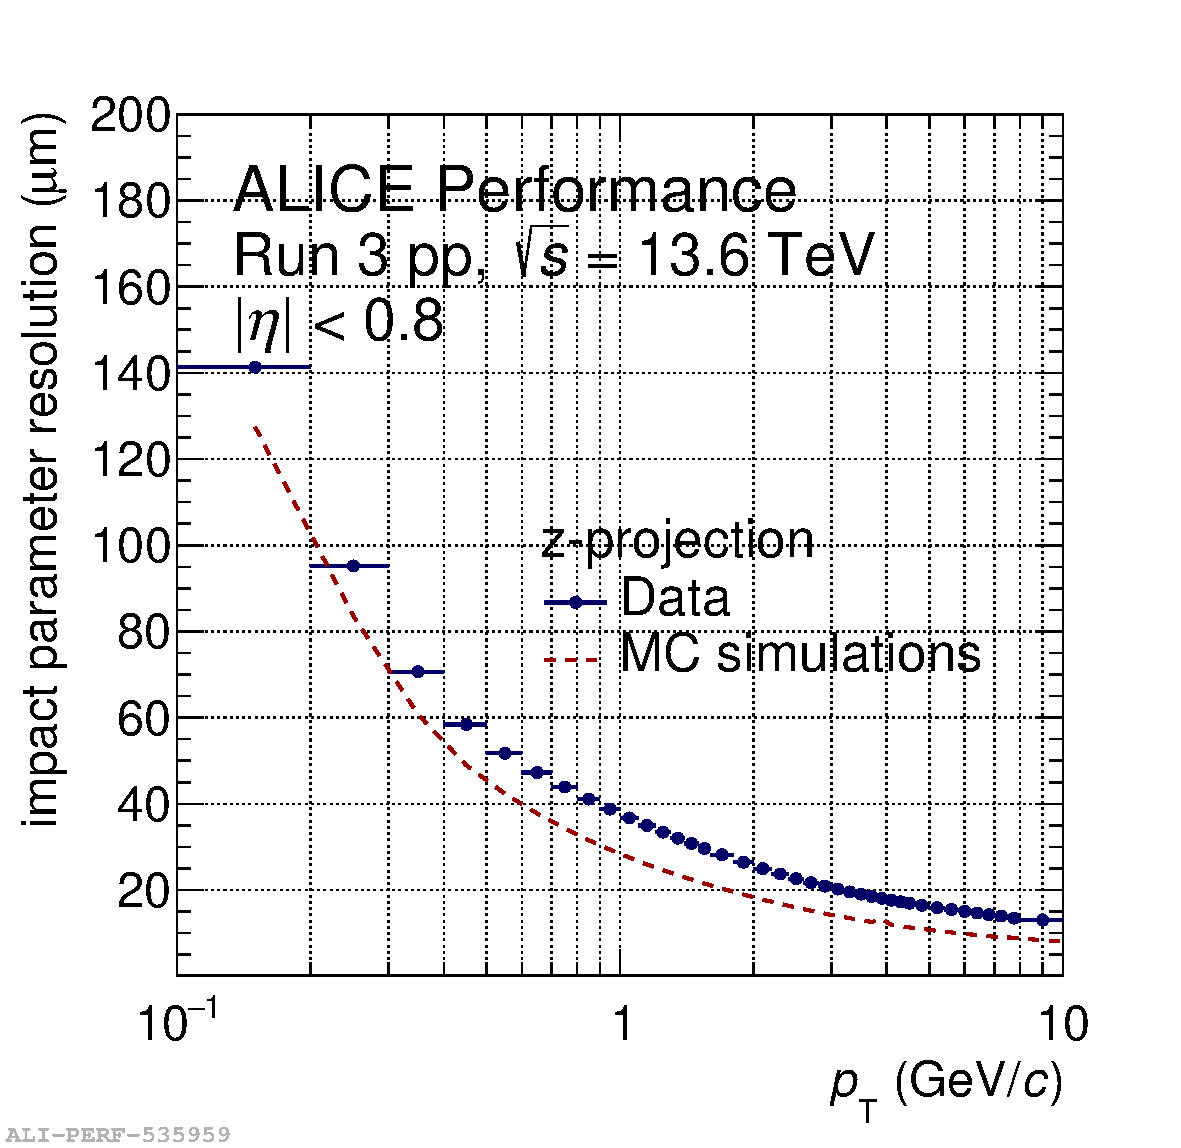
\includegraphics[width=0.48\textwidth]{Figures/Chapter 6/sigmadcaz_lhc22q_pass2_lhcc.pdf}
    \caption{Impact-parameter resolution in the transverse plane (left panel) and beam direction (right panel) of primary particles in data and MC. Figure taken from the ALICE figure repository~\cite{ALICE_figures}.} 
    \label{fig:dca_res} 
    \end{center}
\end{figure}

Special care is taken to ensure that the MC simulation reproduces the experimental conditions and the reconstruction configuration used for data. A slightly worse impact-parameter resolution is obtained in data, probably due to a residual misalignment of the ITS, as shown in Fig.~\ref{fig:dca_res}, where the impact parameter resolutions in the transverse plane and along the beam direction are shown for both data and MC simulations. To improve the MC description of the spatial resolution measured in data, a smearing of the track impact parameters (i.e., the distance of closest approach to the primary vertex) is applied via a dedicated workflow (\code{track-tuner}). The workflow has been tuned by comparing the impact-parameter resolution in data and MC obtained by fitting their distributions for primary particles. The \code{track-tuner} workflow allows the MC simulations to reproduce the impact parameter resolution observed in data.

\begin{figure}[htb]
    \begin{center}
    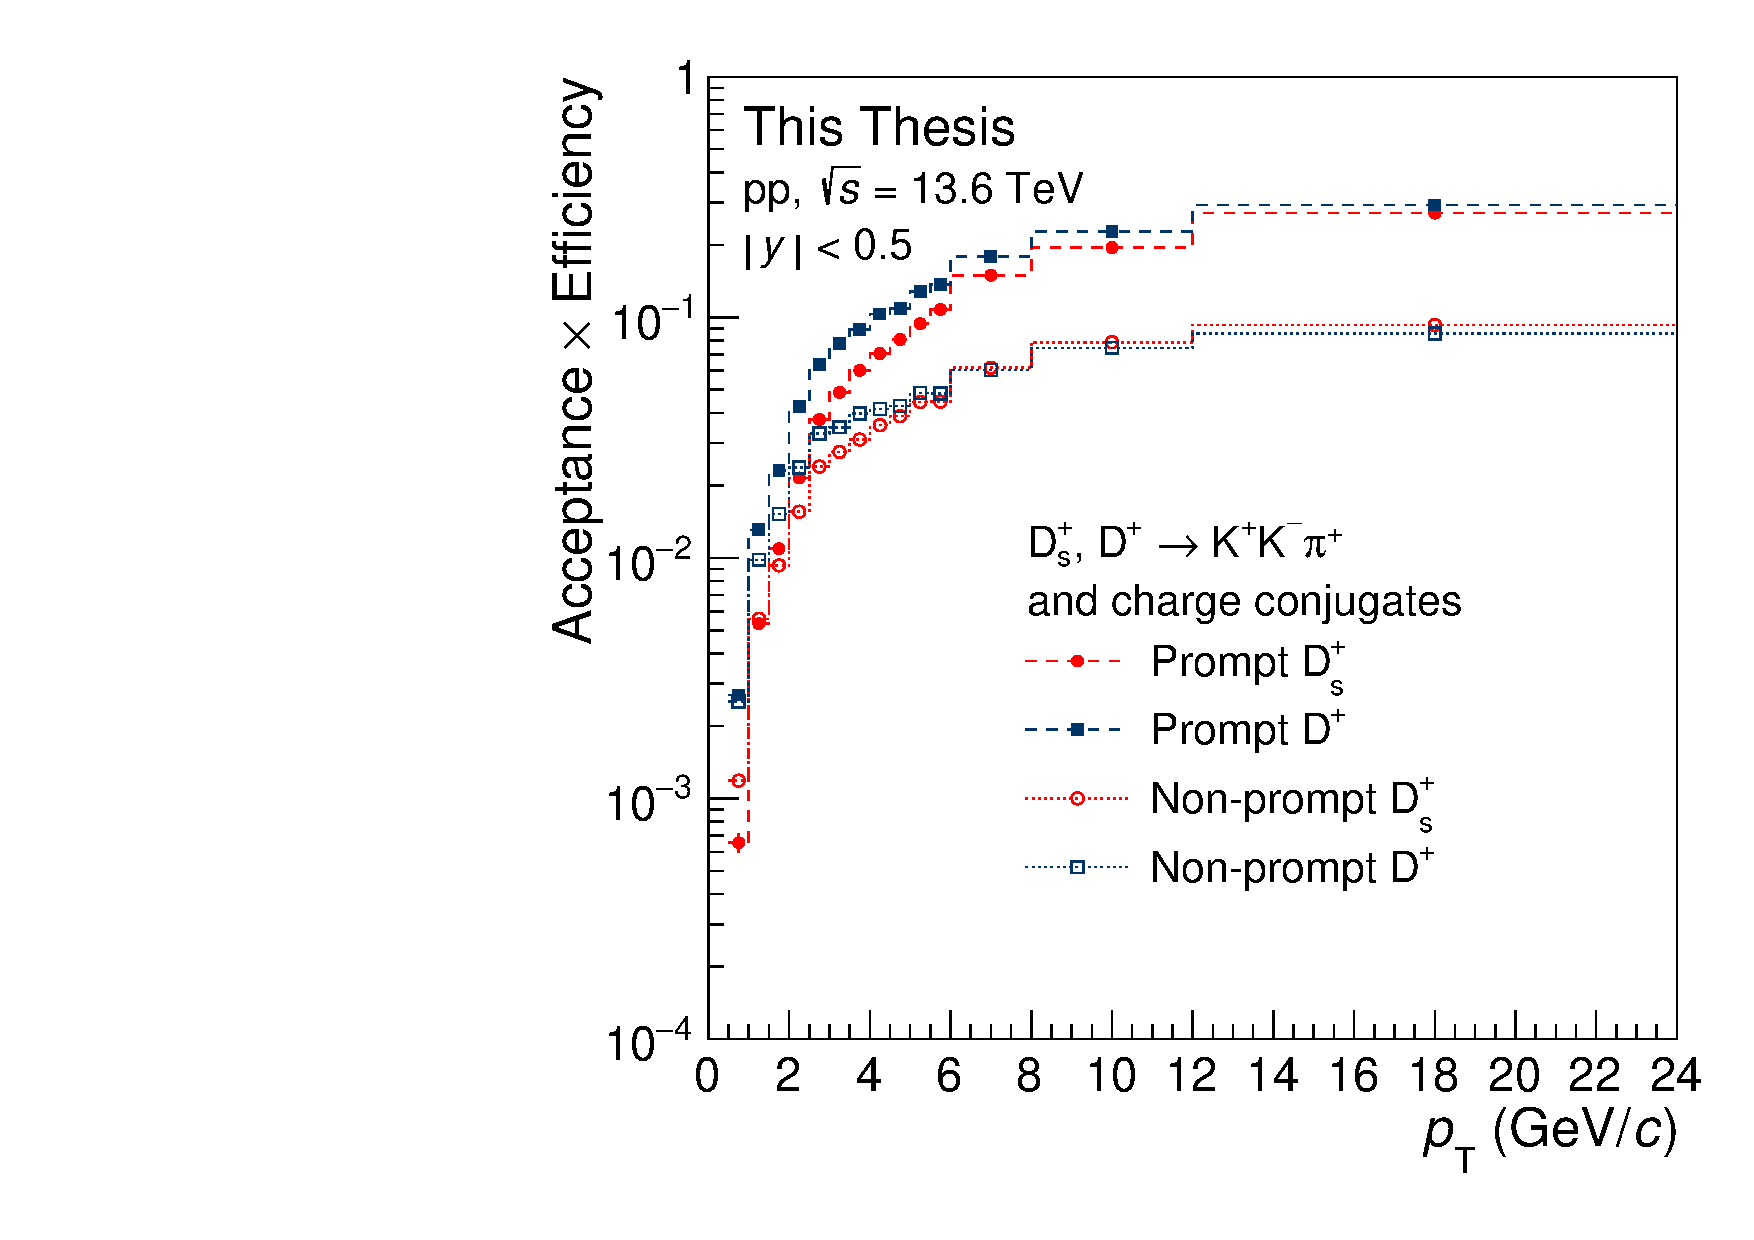
\includegraphics[width=0.7\textwidth]{Figures/Chapter 6/Efficiency_LHC24d3a.pdf}
    \caption{Acceptance-times-efficiency correction factor as a function of \pt for prompt and non-prompt \ds and \dpl mesons.} 
    \label{fig:Aeff} 
    \end{center}
\end{figure}

The \aeff factor is defined as
\begin{equation*}
    \aeff = \frac{N_\mathrm{sel.}^{\lvert y\rvert<0.8}}{N_\mathrm{gen.}^{\lvert y\rvert<0.5}}\quad ,
\end{equation*}
where $N_\mathrm{gen.}^{\lvert y\rvert<0.5}$ is the number of generated D mesons with $\lvert y\rvert<0.5$, and $N_\mathrm{sel.}^{\lvert y\rvert<0.8}$ is the number of D mesons with $\lvert y\rvert<0.8$ that pass the applied selection criteria. The \aeff factor is illustrated in Fig.~\ref{fig:Aeff} for both \ds and \dpl mesons as a function of \pt. Due to the different decay topologies of \ds and \dpl mesons, with the second decaying on average at a larger distance from the primary vertex, the efficiency is lower for \ds mesons than for \dpl mesons, while the acceptance for the two meson species is the same. For the same reason, the \aeff factor is larger for promptly-produced D mesons than for non-prompt ones. The correction presents a strong dependence on \pt. The larger Lorentz boost of D mesons at high \pt results in a more displaced decay vertex, facilitating the selection of \ds and \dpl mesons. To extract a statistically significant signal at low \pt, where a larger number of background tracks (and therefore combinatorial background candidates) is present, the selection criteria are tightened, reducing the efficiency of the selection. The \aeff correction ranges from about 0.3 in the highest \pt interval down to about $7\times 10^{-4}$ in the lowest considered \pt interval.


\section{Prompt fraction correction}\label{sec:fp}
The fraction of prompt \ds and \dpl mesons in the measured raw yield (\fpds and \fpdpl) is estimated using a data-driven method that involves varying the BDT probability threshold for candidate selection. This variation changes the balance between prompt and non-prompt contributions to the signal, exploiting their different trends with the BDT output score to disentangle their relative abundances in the extracted raw yield. Introduced in Ref.~\cite{ALICE:2021mgk}, this approach leverages the relationship between the raw yield and the number of produced prompt ($N_\mathrm{prompt}$) and non-prompt ($N_\mathrm{non\text{-}prompt}$) D mesons decaying into the considered decay channel:
\begin{equation}\label{eq:fp_rawyields}
    N_\mathrm{raw} = N_\mathrm{prompt}\times\aeffp + N_\mathrm{non\text{-}prompt} \times \aeffnp\quad .
\end{equation}
\vspace{0.1cm}
Eq.~\ref{eq:fp_rawyields} holds for every chosen BDT selection criterion, defining the \aeffp and \aeffnp correction factors and the raw yield $N_\mathrm{raw}$. Since the \aeff factors can be determined from MC simulations (as described in the previous section), and $N_\mathrm{raw}$ is extracted through a fit to the invariant mass distribution of selected candidates from data (as detailed in Chapter~\ref{chap:RY}), Eq.~\ref{eq:fp_rawyields} contains only two unknown variables, $N_\mathrm{prompt}$ and $N_\mathrm{non\text{-}prompt}$. They can be evaluated by varying the BDT working point, extracting the corresponding raw yield, and estimating the \aeffp and \aeffnp factors. However, a single variation of the selection criteria may lead to large uncertainties, as a small change in the \aeff correction adds limited information on $N_\mathrm{prompt}$ and $N_\mathrm{non\text{-}prompt}$. To overcome this issue, the BDT threshold values are varied several times to span a wide range of \aeffp (and \aeffnp) and significantly change the \fp (and \fnp) in the extracted raw yield. For each selection criterion i, the acceptance-times-efficiency factor is calculated for prompt $\aeffp^\mathrm{i}$ and non-prompt $\aeffnp^\mathrm{i}$ D mesons, and the raw yields $N_\mathrm{raw}^\mathrm{i}$ are extracted by fitting the invariant mass distribution of candidates passing the selections. By including the entire set of selection criteria, a system of equations can be defined:
\begin{equation*}
    \begin{cases}
        N_\mathrm{raw}^1 = N_\mathrm{prompt}\times\aeffp^1 + N_\mathrm{non\text{-}prompt} \times \aeffnp^1\\
        N_\mathrm{raw}^2 = N_\mathrm{prompt}\times\aeffp^2 + N_\mathrm{non\text{-}prompt} \times \aeffnp^2\\
        \vdots\\
        N_\mathrm{raw}^\mathrm{n} = N_\mathrm{prompt}\times\aeffp^\mathrm{n} + N_\mathrm{non\text{-}prompt} \times \aeffnp^\mathrm{n}
    \end{cases}
    \quad .
\end{equation*}
For $\mathrm{n>2}$, the system of equations is overconstrained, and the solution can be found through a minimisation procedure. The system of equations can be written in matrix notation as
\begin{equation*}
    \begin{pmatrix}
        \aeffp^1 & \aeffnp^1\\
        \aeffp^2 & \aeffnp^2\\
        \vdots & \vdots\\
        \aeffp^\mathrm{n} & \aeffnp^\mathrm{n}
    \end{pmatrix}
    \begin{pmatrix}
        N_\mathrm{prompt}\\
        N_\mathrm{non\text{-}prompt}
    \end{pmatrix}
    -
    \begin{pmatrix}
        N_\mathrm{raw}^1\\
        N_\mathrm{raw}^2\\
        \vdots\\
        N_\mathrm{raw}^\mathrm{n}
    \end{pmatrix}
    =
    \begin{pmatrix}
        \delta^1\\
        \delta^2\\
        \vdots\\
        \delta^\mathrm{n}
    \end{pmatrix}
    \quad ,
\end{equation*}
where $\delta^\mathrm{i}$ are the residuals due to the uncertainty in the raw yield and \aeff correction factors for the i-th selection. For each selection criterion, the uncertainty on $\delta^\mathrm{i}$ is estimated by propagating the uncertainties on the raw yield and \aeff factors as
\begin{equation*}
    \sigma_\mathrm{i}^2 = \sigma_{N_\mathrm{raw}^\mathrm{i}}^2 + N_\mathrm{prompt}\times\sigma^2_{\aeffp^\mathrm{i}} + N_\mathrm{non\text{-}prompt}\times\sigma^2_{\aeffnp^\mathrm{i}}\quad ,
\end{equation*}
where $\sigma_{N_\mathrm{raw}^\mathrm{i}}$ is the uncertainty on the extracted raw yield, and $\sigma_{\aeffp^\mathrm{i}}$ and $\sigma_{\aeffnp^\mathrm{i}}$ are the uncertainties on the prompt and non-prompt \aeff factors, respectively. Given that the corrected prompt and non-prompt yields are unknown variables, an iterative procedure is used to define the total uncertainty: initially, $N_{\mathrm{prompt}}$ and $N_{\mathrm{non\text{-}prompt}}$ are set to zero and only the uncertainty on the raw yields is taken into account (as $\sigma_{\aeffp^\mathrm{i}}$ and $\sigma_{\aeffnp^\mathrm{i}}$ are not relevant in the evaluation of $\sigma_\mathrm{i}$ if $N_\mathrm{prompt}=N_\mathrm{non\text{-}prompt}=0$). From the second iteration, the corrected yields $N_{\mathrm{prompt}}$ and $N_{\mathrm{non\text{-}prompt}}$ obtained in the previous step are also used, along with the uncertainties on the \aeff factors. This iteration is repeated until the difference between the corrected yields in successive iterations falls below a predefined threshold.

The solution of the system of equations is found by minimising the residuals with a least-squares method, with a $\chi^2$ defined as 
\begin{equation*}
    \chi^2 = \pmb{\delta}^\mathrm{T}\mathbf{C}^{-1}\pmb{\delta}\quad ,
\end{equation*}
where $\pmb{\delta}$ is the vector of residuals and $\mathbf{C}$ is the covariance matrix of the residuals.

In this analysis, the BDT threshold is fixed for the background score, at a tighter value than the one used to extract the central raw yields to ensure the convergence of the invariant mass fits. The minimum probability for being a non-prompt D meson is varied in different ranges for the two D meson species, to guarantee that a large enough variation in the \fnp is achieved. Indeed, due to the larger proper mean decay length of \dpl mesons, the usage of the selection criteria employed for the \ds meson would lead to a smaller variation in the \fnp factor for the \dpl meson. Therefore, the BDT threshold for the non-prompt score is varied in a wider range for \dpl mesons than for \ds mesons, reaching larger threshold values on the minimum non-prompt BDT score for \dpl mesons. 

Because the selection criterion is increasingly tightened, the $\mathrm{i+1}$-th selected sample will be entirely contained in the $\mathrm{i}$-th one. The residuals $\delta^\mathrm{i}$ will therefore exhibit a degree of correlation. The off-diagonal element $\sigma_\mathrm{i,j}$ of the covariance matrix $\mathbf{C}$, i.e., the covariance between the residuals of the i-th and j-th selection criteria, can be estimated as 
\begin{equation*}
    \sigma_\mathrm{i,j} = \rho_\mathrm{i,j}\sigma_\mathrm{i}\sigma_\mathrm{j}\quad ,
\end{equation*}
where it can be demonstrated~\cite{cowan1998statistical} that the correlation coefficient $\rho_\mathrm{i,j}$ is given by 
\begin{equation*}
    \rho_\mathrm{i,j} = \frac{\sigma_\mathrm{i}}{\sigma_\mathrm{j}}\quad 
\end{equation*}
if the measurement i is made on a dataset that is fully included in the one used for the measurement j. 

The minimisation procedure described above leads to the determination of the true number of prompt and non-prompt D mesons decaying into the considered decay channel ($N_\mathrm{prompt}$ and $N_\mathrm{non\text{-}prompt}$, respectively), which are independent of the applied selection criteria. The results for the evaluation of the \fpds correction factor in the $1.5<\pt<2.0$~\gevc interval are shown in Fig.~\ref{fig:fp}. The complete set of figures on the results of the evaluation of the \fpds and \fpdpl factors is provided in Appendix~\ref{app:fpds}. In the top-left panel, the correlation factor $\rho$ between the residuals $\delta^\mathrm{i}$ is shown for the different selection criteria; in the top-right panel, the \aeff factors are shown for both prompt and non-prompt \ds mesons as a function of the index used to refer to the BDT threshold value applied to the non-prompt BDT output score. The leftmost data point of each distribution corresponds to the loosest selection on the BDT non-prompt score, while the rightmost one corresponds to the strictest selection, which is expected to preferentially select non-prompt D mesons. In the bottom-left panel, the relative contribution of the prompt and non-prompt components to the extracted \ds raw yields is shown as a function of the ML selections. Lastly, in the bottom-right panel, the extracted yields are fitted using a template fit, utilising the \aeffpds and \aeffnpds evolution as a function of the BDT selection criterion. The minimisation procedure described above can in fact be interpreted as a template fit to the extracted raw yields, where the templates are the \aeff factors as a function of the BDT selection. The prompt and non-prompt components of the raw yield, obtained for each BDT-based selection from the minimisation procedure as \mbox{$\aeffp\times N_\mathrm{prompt}$} and $\aeffnp\times N_\mathrm{non\text{-}prompt}$ respectively, are represented with red and blue filled histograms. Their sum is reported by the green histogram. Given the small $\chi^2$/ndf value obtained from the fit, the \fp factor is considered to be well determined. 
\begin{figure}[htb]
    \begin{center}
    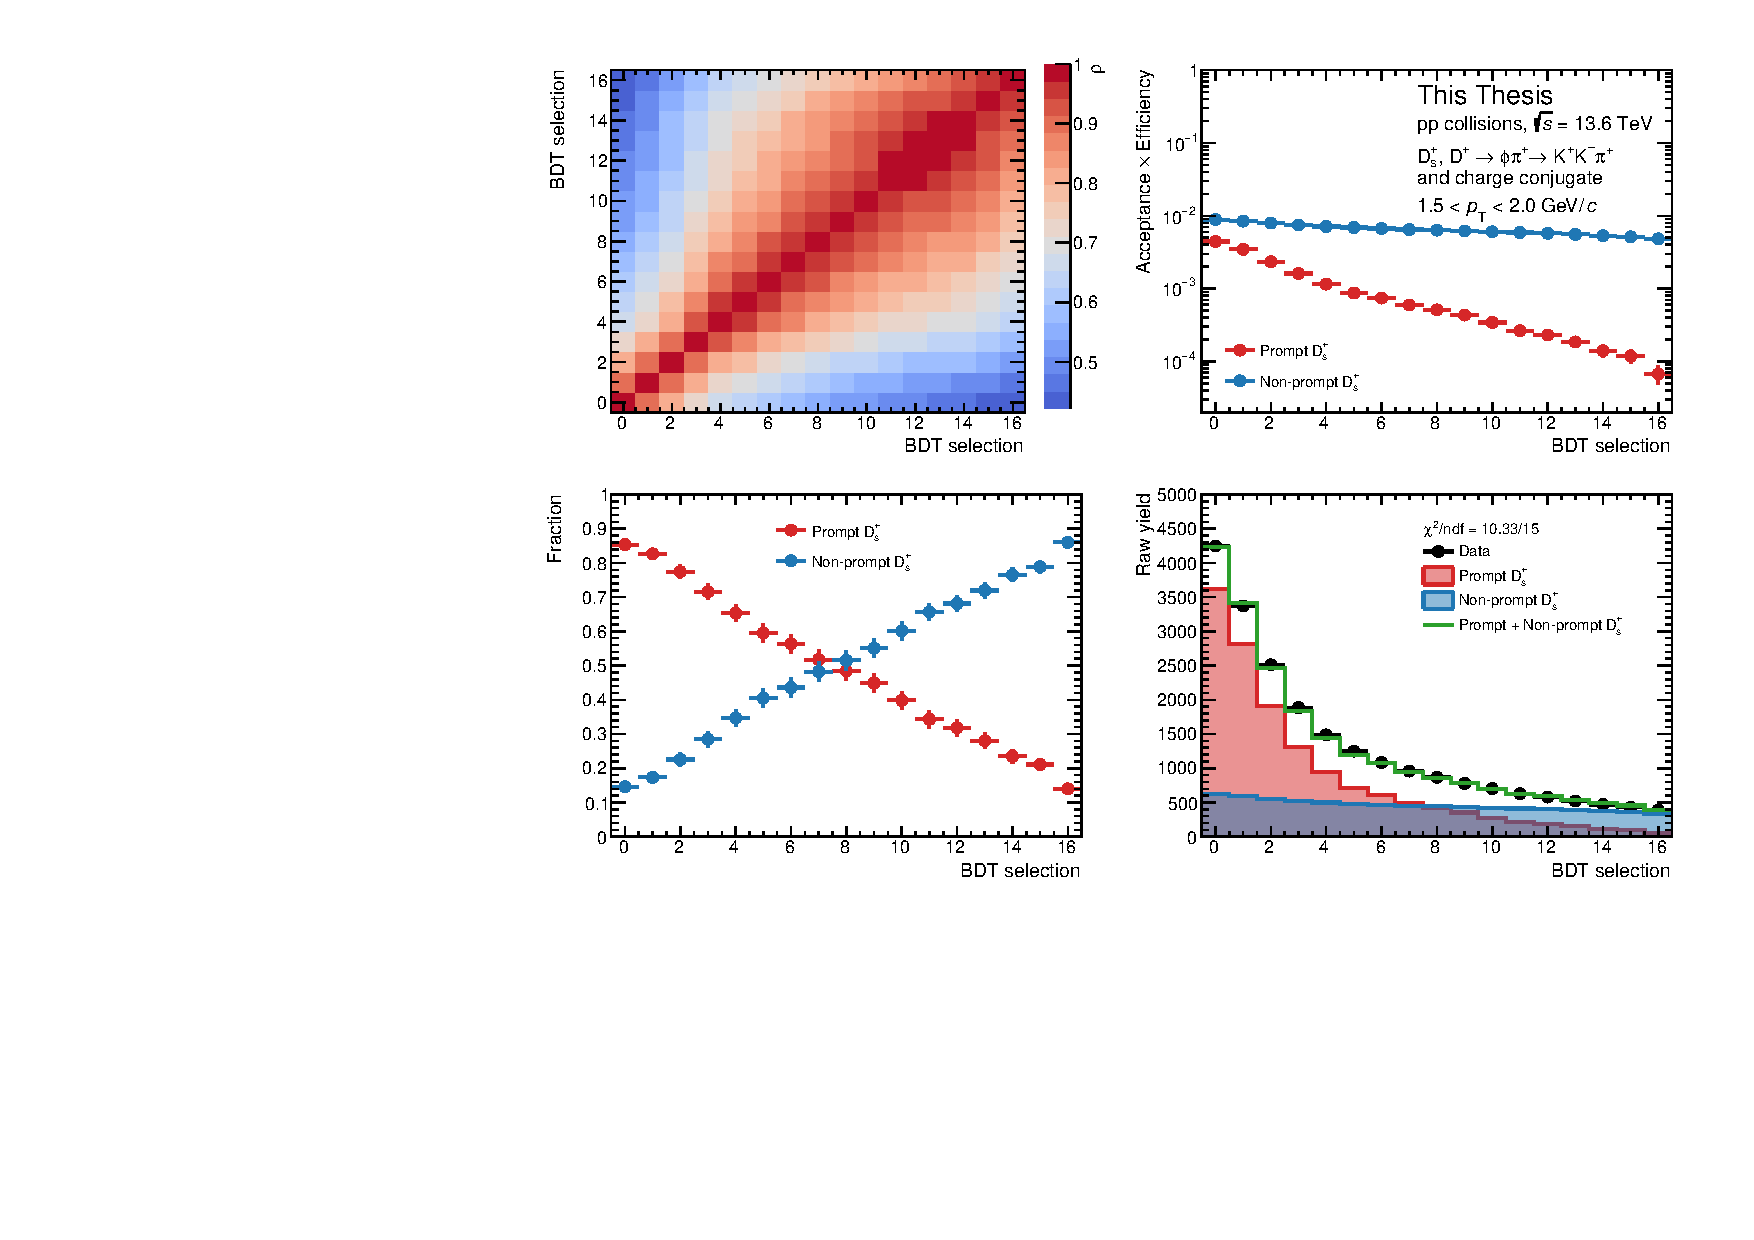
\includegraphics[width=\textwidth]{Figures/Chapter 6/DsPromptFrac.pdf}
    \caption{Results for the evaluation of the \ds \fp correction factor in the \mbox{$1.5<\pt<2.0$~\gevc} interval. The correlation factor $\rho$ (top-left panel), \mbox{\aeff} factors for both prompt and non-prompt \ds mesons (top-right panel), prompt and non-prompt fraction in the extracted \ds raw yields (bottom-left panel), and contribution of prompt and non-prompt \ds mesons to the extracted raw yields (bottom-right panel) are shown for the different BDT selection criteria applied on the non-prompt probability.} 
    \label{fig:fp} 
    \end{center}
\end{figure}

The \fp factor is then calculated for each D-meson species and for any given selection criterion with efficiencies \aeffp and \aeffnp for prompt and non-prompt D mesons respectively, as
\begin{equation*}
    \fp = \frac{N_\mathrm{prompt}\times\aeffp}{N_\mathrm{prompt}\times\aeffp + N_\mathrm{non\text{-}prompt}\times\aeffnp}\quad .
\end{equation*}

As a cross-check, the \fp factor is also estimated using a theory-driven approach~\cite{ALICE:2017olh}, which relies on FONLL~\cite{Cacciari:1998it} predictions for beauty-hadron production and the decay kinematic description of \textsc{Pythia~8}~\cite{Bierlich:2022pfr} for estimating the \pt differential cross section of non-prompt D mesons. The \fp factor is then calculated for each D-meson species as 
\begin{equation*}
    \fp = 1-\left.\frac{\de^2\sigma}{\de\pt\de y}\right\vert_\mathrm{FONLL+\textsc{Pythia}~8}^\mathrm{non\text{-}prompt}\times\frac{\aeffnp \Delta y \Delta\pt \mathrm{BR} \mathcal{L}_\mathrm{int}}{\frac{1}{2}\times N_\mathrm{raw} }\quad ,
\end{equation*}
where $\Delta y$ and $\Delta\pt$ are the rapidity and \pt intervals, respectively, $\mathcal{L}_\mathrm{int}$ is the integrated luminosity of the data sample, which is \SI{1}{\per\pico\barn}, $N_\mathrm{raw}$ is the extracted raw yield of the considered D meson species, and the factor 1/2 takes into account that both particle and antiparticles are selected, while FONLL calculations include only particles. The uncertainty on the \fp factor is propagated through a Gaussian approach, taking into account the uncertainties on the FONLL predictions, raw yield, and \aeffnp factor. 

A comparison between the \fp correction factors for \ds and \dpl mesons in the different \pt intervals of the anlaysis obtained with the two methods is illustrated in the left panel of Fig.~\ref{fig:fp_comparison}. A good level of agreement is observed between the two results, which are compatible within their uncertainties across the studied \pt range, with the exception of the highest \pt interval, where fluctuations in the yield extraction with the data-driven method lead to a small discrepancy between the two methods. For the evaluation of the central \fp values, the data-driven method is used, as it is not sensitive to possible shortcomings in the theoretical description of $\mathrm{b\overline{b}}$ production from FONLL which may affect the theory-driven approach. The \fp factors result to be larger for \dpl mesons than for \ds mesons, although being compatible within uncertainties. This is due to the larger mean proper decay length of the former, which results in a larger fraction of non-prompt D mesons in the extracted raw yield, as the selection of signal candidates is based on the displaced decay topology. Additionally, the \fp correction factor is found to be almost constant as a function of \pt. This differs from the ``natural'' (corrected) prompt fraction of the two D-meson species, which can be estimated as $N_\mathrm{prompt}/(N_\mathrm{prompt}+N_\mathrm{non\text{-}prompt})$ using the data-driven approach described above, reported in the right panel of Fig.~\ref{fig:fp_comparison}. A decreasing trend with \pt is present in the corrected prompt fraction for both \ds and \dpl mesons. The different trend with \pt of the \fp correction factor as compared to the corrected \fp factor is due to the BDT selection criteria, which are loosened at high \pt and more promptly produced D mesons are selected.

\begin{figure}
    \begin{center}
    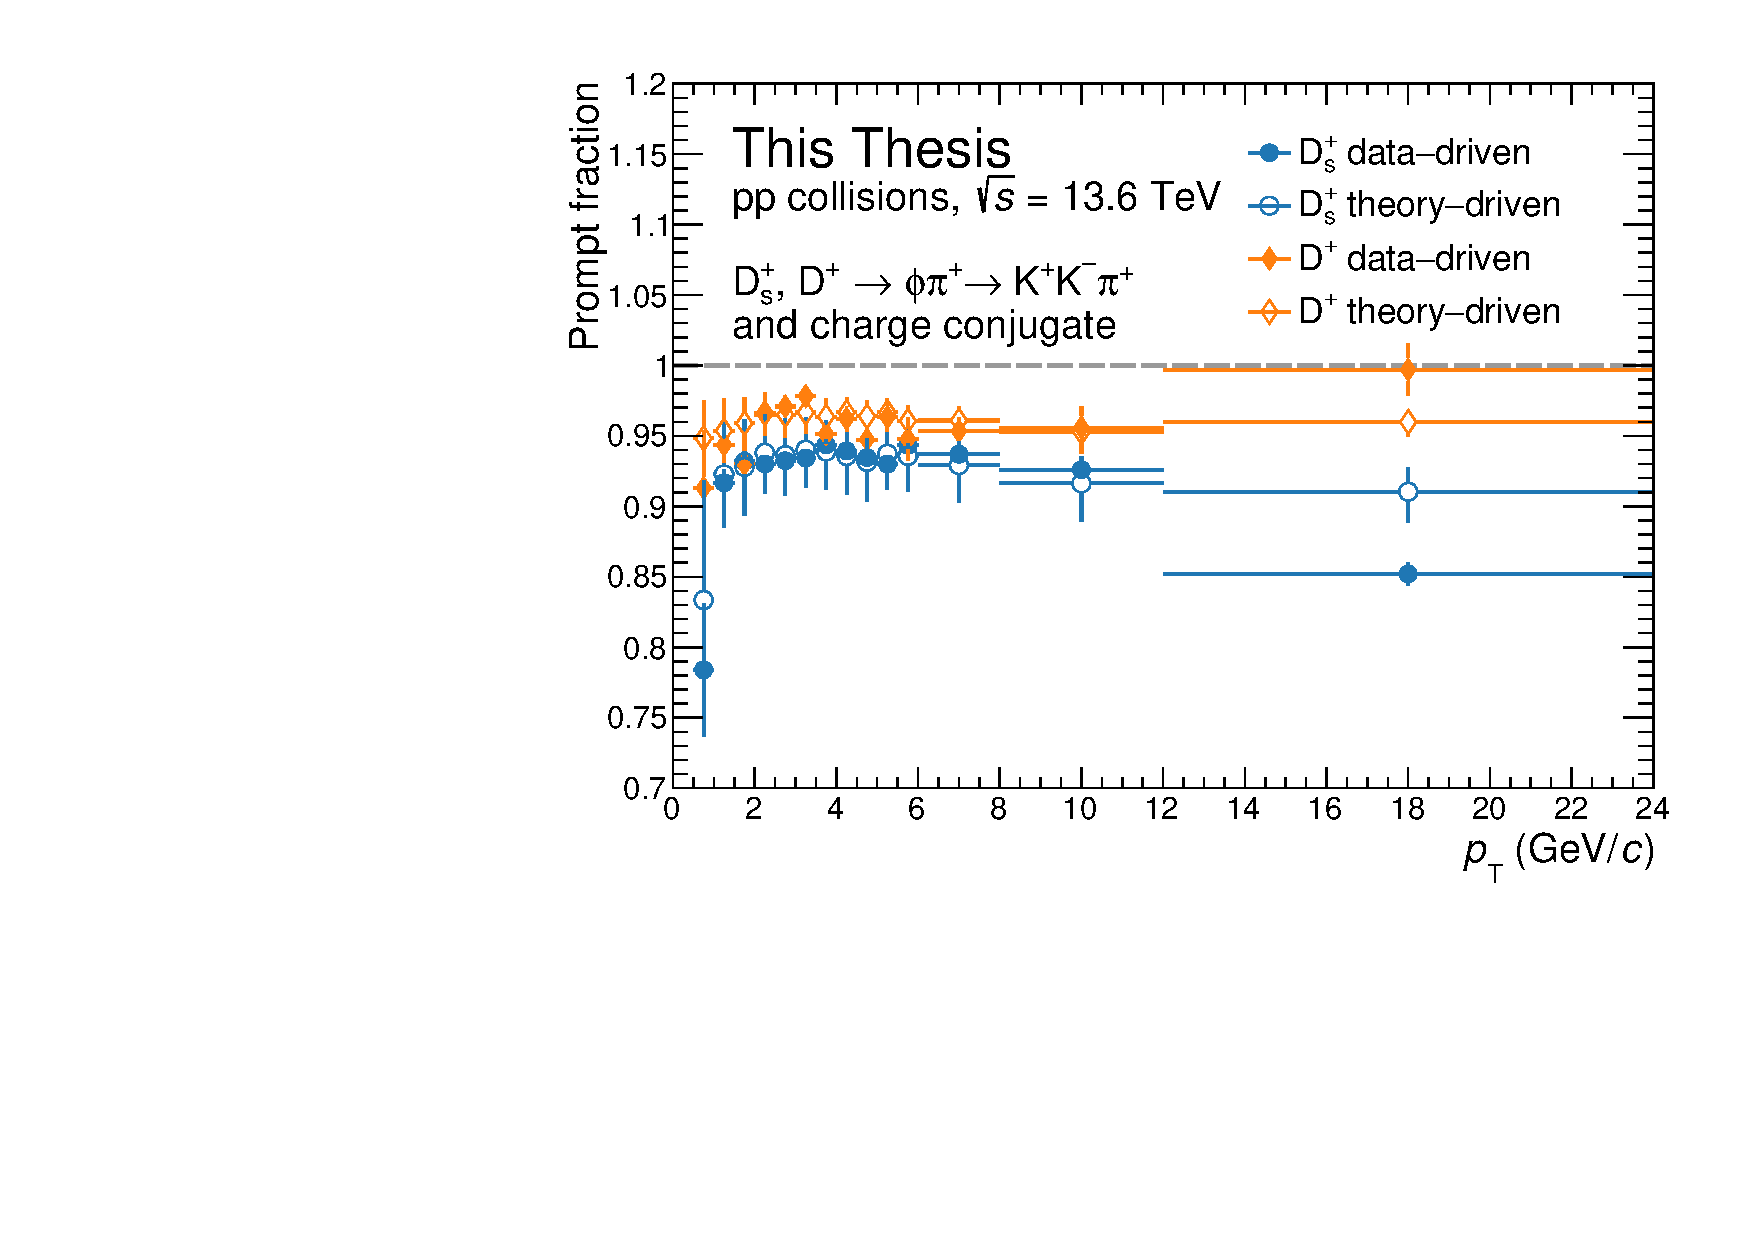
\includegraphics[width=0.48\textwidth]{Figures/Chapter 6/Compare_data_theory_frac.pdf}
    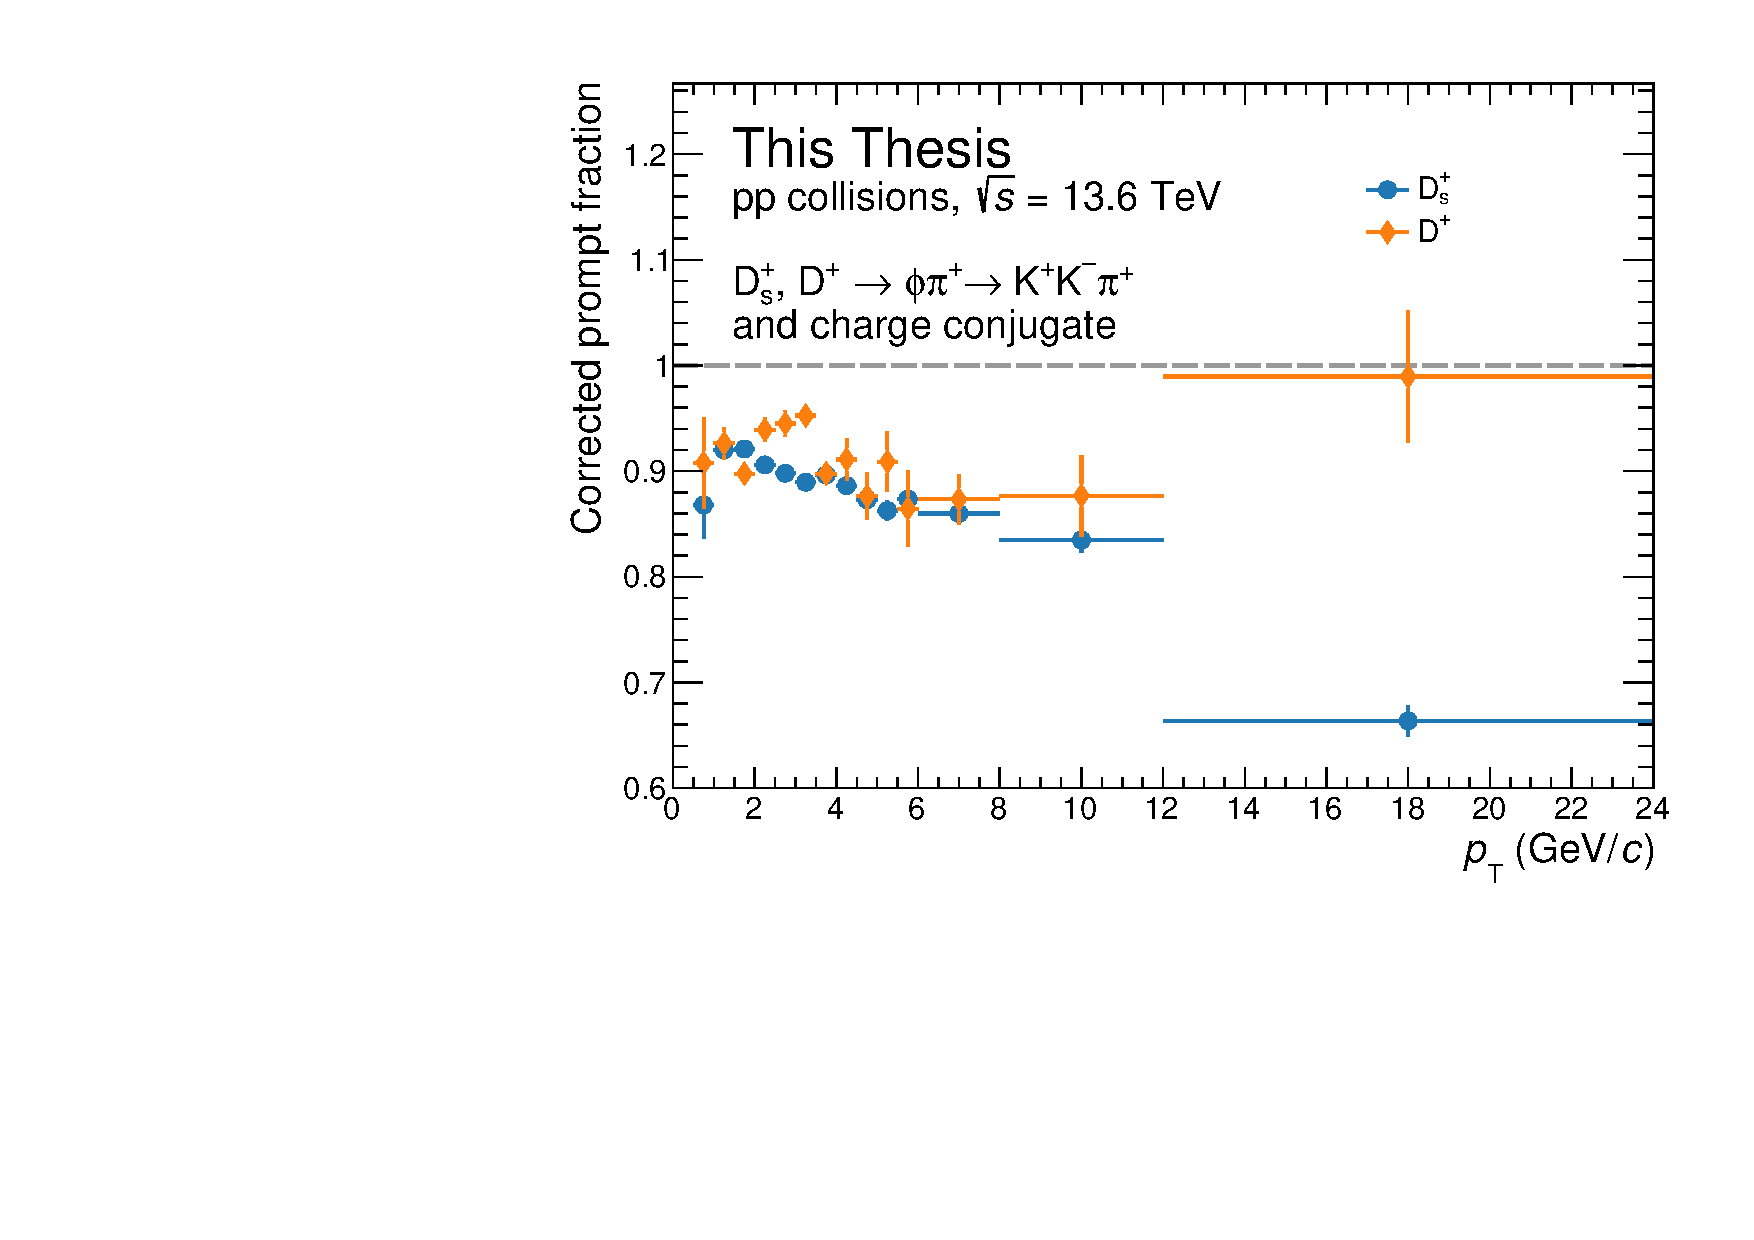
\includegraphics[width=0.48\textwidth]{Figures/Chapter 6/Compare_prompt_frac.pdf}
    \caption{Left panel: \fp correction factor for \ds (blue) and \dpl (orange) mesons as a function of \pt. The results obtained with the data-driven (filled markers) method are compared with those exploiting a theory-driven approach (void markers). Right panel: corrected \fp factors for \ds (blue) and \dpl (orange) mesons as a function of \pt, obtained with the data-driven method.} 
    \label{fig:fp_comparison} 
    \end{center}
\end{figure}

\section{Branching ratio correction}
\begin{sloppypar}

The branching ratio correction is applied to account for the fact that of the produced \ds and \dpl mesons, only those decaying into a $\phi\pi^+\rightarrow\mathrm{K^+K^-\pi^+}$ final state are reconstructed. The values of the branching ratios for the considered decays are taken from Ref.~\cite{pdg}, and correspond to \mbox{$\mathrm{BR}(\ds) = (2.21\pm0.06)\times10^{-2}$} and \mbox{$\mathrm{BR}(\dpl) = \left((2.69^{+0.07}_{-0.08})\times10^{-3}\right)$}. The uncertainty, taken from the PDG, is propagated to the \ds/\dpl production yield ratio with a Gaussian approach, yielding an asymmetric $^{+3.7}_{-4.0}\%$ uncertainty on the ratio.
\end{sloppypar}

\section{Systematic uncertainties}
Measurements of ratios between different particles' production yields allow for the cancellation of some of the systematic uncertainties that have to be taken into account for the measurement of production cross sections, such as that related to luminosity. In addition, the reconstruction of \ds and \dpl mesons through the same decay channel allows for the cancellation of supplementary sources of systematic uncertainties, such as those related to tracking and PID efficiency, thereby enhancing the precision of the results. Nonetheless, the measurement is still affected by several sources of systematic uncertainties, due to arbitrary choices made in the analysis, or the need to rely on MC simulations, which could not perfectly reproduce the data. 

The first systematic uncertainty, related to the extraction of the \ds- and \dpl-meson raw yields, has already been discussed in Chapter~\ref{chap:RY}. In the next sections, other sources of systematic uncertainty, related to the correction factors presented above, are discussed.

\subsection{BDT selection efficiency}\label{sec:BDT_syst}
The choice of the set of BDT threshold values used to extract the raw yields is arbitrary, albeit driven by a defined criterion through the optimisation of the significance on a subsample of the analysed dataset. Variations in the ML selection criteria may lead to differences in the extracted raw yields, and therefore in the \ds/\dpl production yield ratio, due to possible imperfections in the MC description of the topological, kinematic, and PID variables used in the training of the BDT model. The systematic uncertainty on the BDT selection efficiency is assessed by repeating the analysis varying the BDT threshold values on prompt and background probabilities, independently and then simultaneously, for a total of 48 variations. Three tighter and three looser BDT thresholds on both the background and prompt D meson scores are used on top of those employed for the central case. To avoid extreme variations in the selection criteria, the \aeffp for both D-meson species is required to be within 30\% of that obtained for the central selections. In addition, to ensure a good fit quality, the $\chi^2$/ndf of the invariant mass fits is required to be below 2, and the statistical significance of the extracted signal is required to be larger than 3 and than half of that obtained with the central selections, for both \ds and \dpl mesons. 

\begin{figure}[h!]
    \begin{center}
    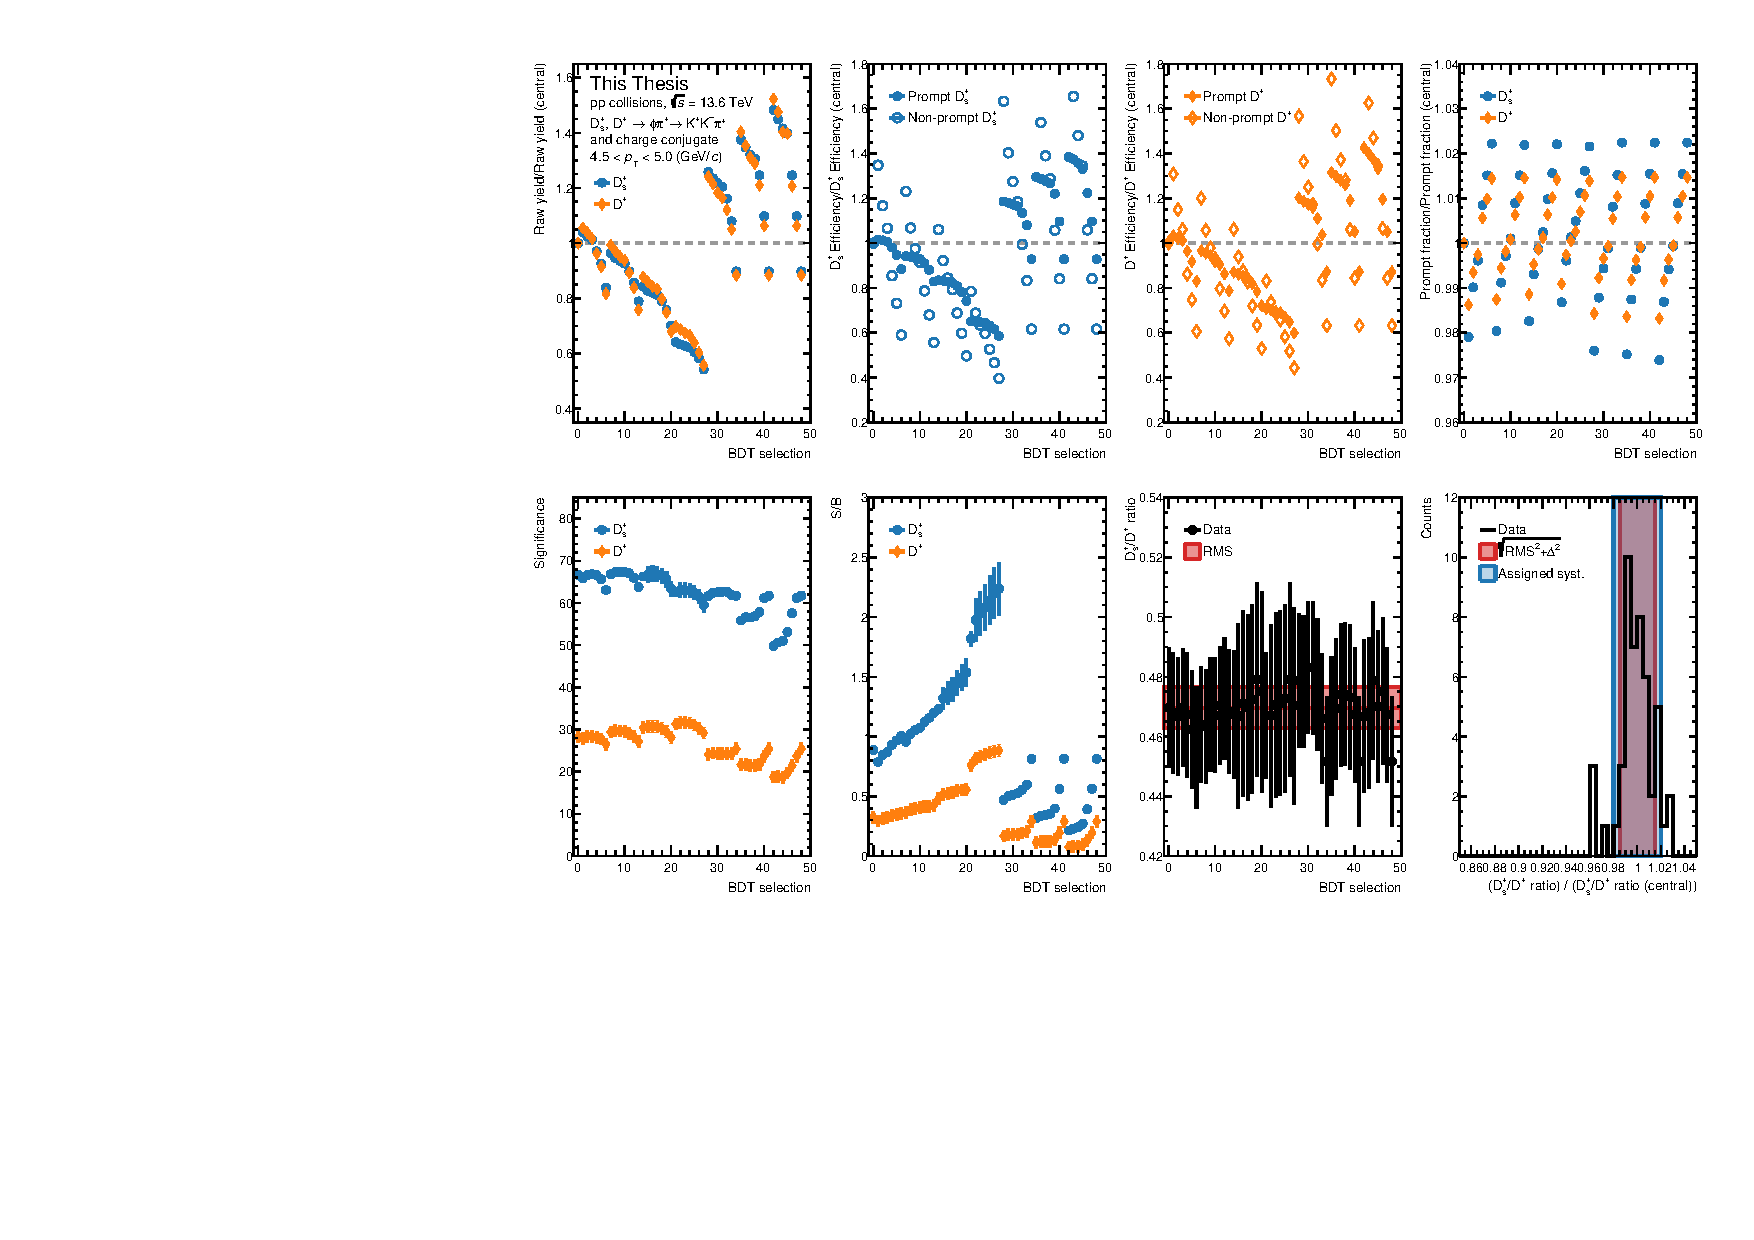
\includegraphics[width=\textwidth]{Figures/Chapter 6/BDTsyst.pdf}
    \caption{Results for the evaluation of the systematic uncertainty on the BDT selection efficiency for the \mbox{$4.5<\pt<5.0$~\gevc} \pt interval. In the top row, the raw yields of \ds (blue) and \dpl (orange) mesons, the prompt (filled markers) and non-prompt (void markers) \ds selection efficiency, the prompt and non-prompt \dpl selection efficiency, and the prompt fraction of \ds and \dpl mesons are shown for the different BDT selections used to estimate the systematic uncertainty, normalised to their respective central values. In the bottom row, the statistical significance of the \ds and \dpl extracted signals, the signal-over-background ratio for the two meson species, and the \ds/\dpl production yield ratio are reported for the different BDT selections. A red band is shown in this last panel around the central value, whose width represents the RMS of the measurements. The rightmost bottom panel shows the distribution of the \ds/\dpl production yield ratio for the different BDT selections divided by the central value. A red band is shown around the central value, representing the sum in quadrature of the standard deviation of the \ds/\dpl distribution and of the difference between its mean and the default value. The blue band displays the assigned systematic uncertainty.} 
    \label{fig:BDT_efficiency} 
    \end{center}
\end{figure}

The results for the estimation of the systematic uncertainty on the BDT selection efficiency are shown in Fig.~\ref{fig:BDT_efficiency} for the \mbox{$4.5<\pt<5.0$~\gevc} \pt interval.  The complete set of figures on the results of the evaluation of the BDT selection efficiency systematic uncertainty is provided in Appendix~\ref{app:bdt}. In the top row, the raw yields of \ds and \dpl mesons, the prompt and non-prompt \ds selection efficiency, the prompt and non-prompt \dpl selection efficiency, and the prompt fraction of \ds and \dpl mesons are shown for the different BDT selections used to estimate the systematic uncertainty, normalised to their respective central values. In the bottom row, the statistical significance of the \ds and \dpl extracted signals, the signal-over-background ratio for the two meson species, and the \ds/\dpl production yield ratio are reported for the considered BDT selections. The different results are ordered such that the central value is the leftmost one (BDT selection 0). In the following six variations, the background score threshold is fixed to the central case, while the prompt score threshold is varied through the whole set of considered values. Then, in the next 21 variations, three different tighter thresholds are applied to the background score, while the prompt score is varied. The last 21 variations are obtained by applying three looser thresholds to the background score and varying the prompt score. In the rightmost bottom panel, the distribution of the \ds/\dpl production yield ratio for the different BDT selections divided by the central value is shown. The systematic uncertainty on the BDT selection efficiency is estimated as the sum in quadrature of the standard deviation of the \ds/\dpl distribution and of the difference $(\Delta)$ between its mean and the value of the ratio obtained with the default selections. The relative uncertainty is then rounded to the nearest 1\% value, and to avoid the inclusion of statistical fluctuations in the assigned systematic uncertainty, the \pt dependence of the systematic uncertainty is smoothed. The assigned systematic uncertainty is reported in Table~\ref{tab:recapSyst} and ranges from 1\% to 10\% depending on \pt. At low \pt, where the efficiency is lower and the sensitivity to possible shortcomings in the MC description of data increases, the uncertainty is larger, reaching 10\% in the lowest \pt interval. The uncertainty then follows a decreasing trend with \pt, reaching 2\% in the highest \pt intervals.

\begin{figure}[tb]
    \begin{center}
    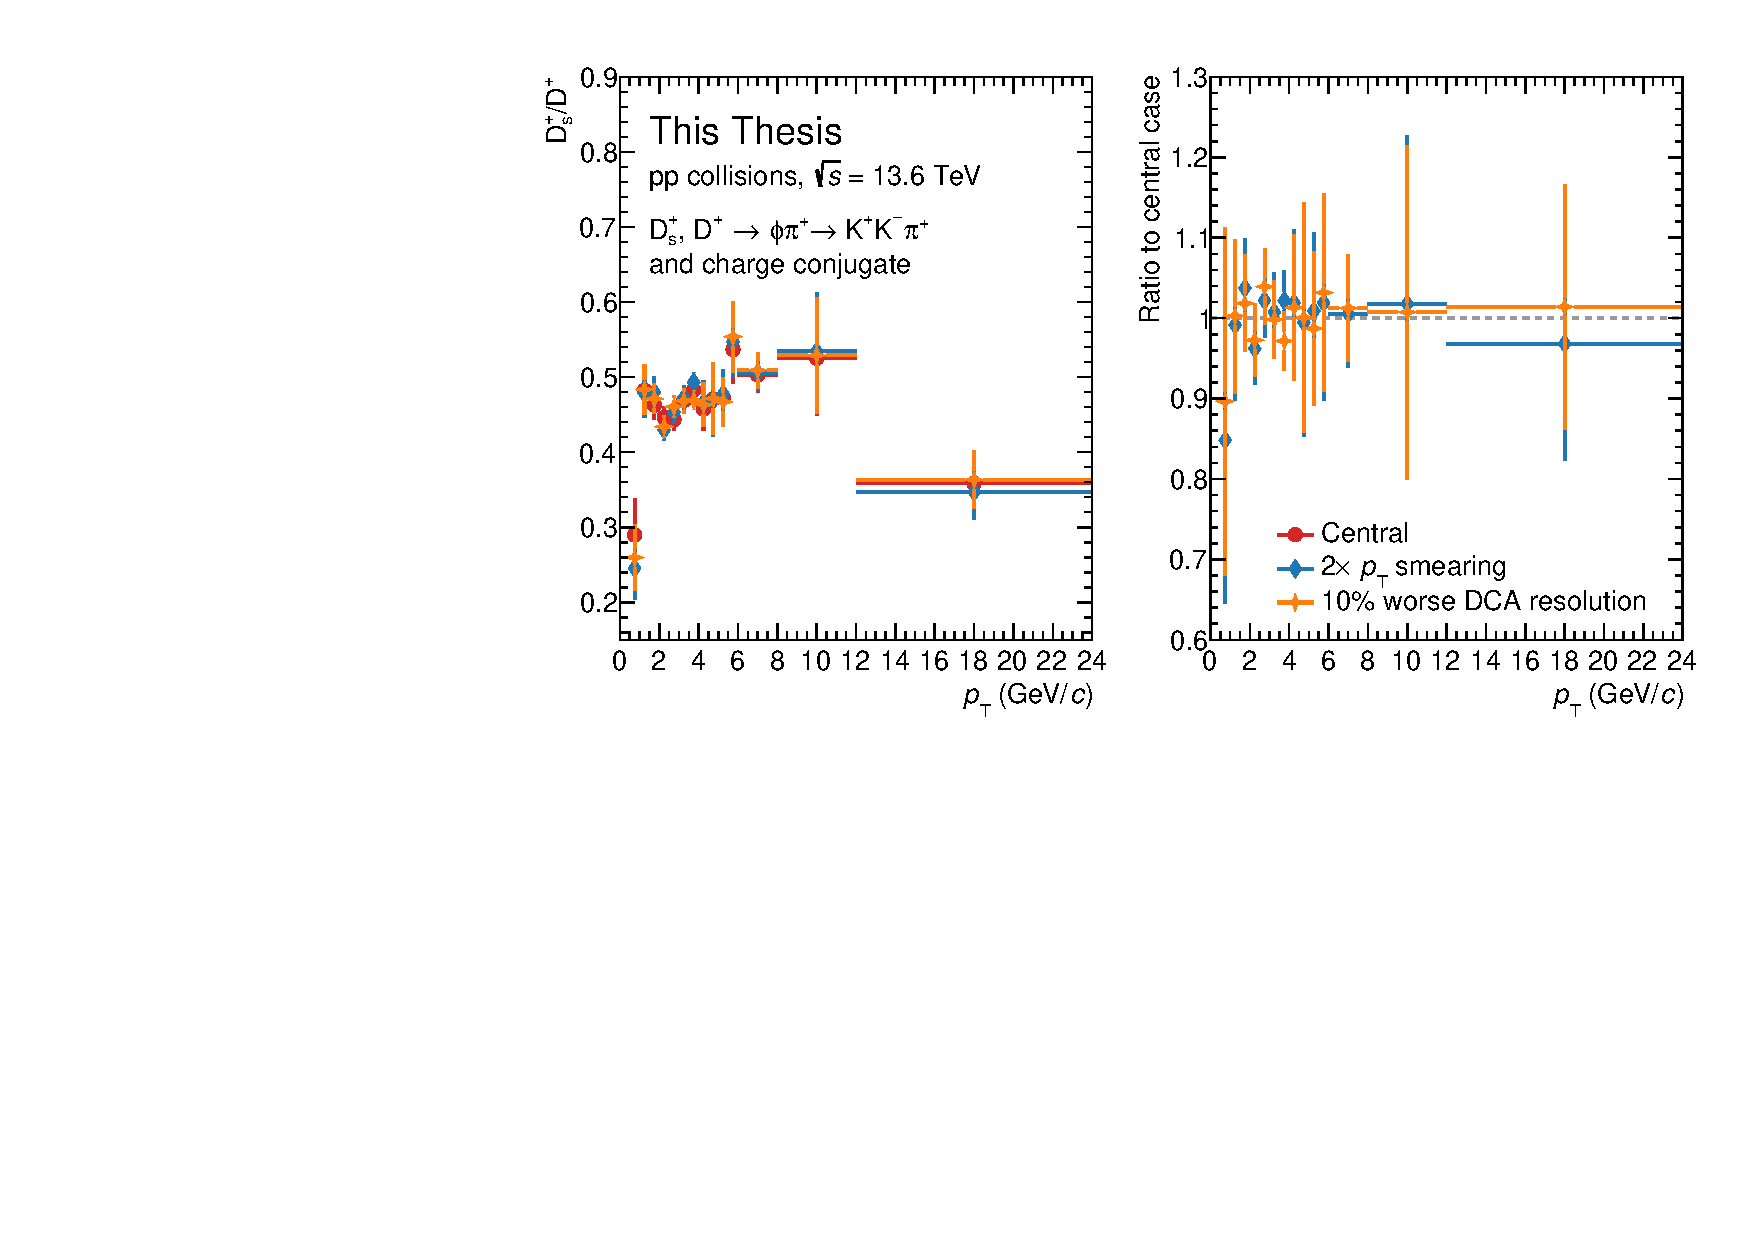
\includegraphics[width=\textwidth]{Figures/Chapter 6/TrackTunerSyst.pdf}
    \caption{Results for the evaluation of the systematic uncertainty on a possible imperfect description of the tracking performance in MC simulations. The \ds/\dpl production yield ratio is shown in the left panel for the central result (red) and for the two different configurations of the \code{track-tuner}: with a factor 2 worse \pt resolution (blue) and a 10\% worse resolution on the track impact parameter (distance of closest approach (DCA), orange). In the right panel, the ratio of the different \ds/\dpl factors to that obtained in the central case is reported.} 
    \label{fig:tracktuner} 
    \end{center}
\end{figure}
\subsection{Imperfections in the description of the tracking performance}
As discussed above, an imperfect description of the topological variables in the MC simulations may imply a systematic uncertainty in the determination of the selection efficiencies of \ds and \dpl mesons. A contribution to this uncertainty was tested by varying the topological selections applied and evaluating the stability of the result against the variations, as discussed in Sec.~\ref{sec:BDT_syst}. In addition to this, the sensitivity of the measurement to possible discrepancies in the impact parameter resolution between data and MC was evaluated by using different configurations of the \code{track-tuner} workflow. In particular, a configuration with a 10\% worse resolution than the default one was considered. Moreover, a version of the \code{track-tuner} implementing a smearing of the track \pt at the innermost update point was also used. In this case, a factor 2 worse \pt resolution was used to account for the discrepancy between the widths of the \ds- and \dpl-meson mass peaks in data and MC. The analysis was repeated using the two different configurations of the \code{track-tuner} for estimating the correction factors, and the resulting \ds/\dpl production yield ratios are shown in Fig.~\ref{fig:tracktuner}, together with the ratio to the central result. The systematic uncertainty is estimated for each \pt interval as the semi-dispersion of the three results. As for the other sources of systematic uncertainty, the \pt dependence of the systematic uncertainty is smoothed. The assigned systematic uncertainty is reported in Table~\ref{tab:recapSyst}, and ranges from 1\% to 8\% depending on \pt. It is maximum at low \pt, where possible imperfections in the MC simulations have a larger impact on the measurement, and decreases with increasing \pt.

\subsection{Prompt fraction}
The choice of the set of selection criteria employed for evaluating the \fp correction via the data-driven procedure described in Sec.~\ref{sec:fp} may introduce a systematic uncertainty on the \ds/\dpl production yield ratio, due to possible imperfections in the description of the efficiency evolution as a function of the applied selections. To estimate the magnitude of this uncertainty, the \fp correction is evaluated using different sets of BDT threshold values. Of the 17 variations on the non-prompt score threshold used to estimate the prompt fraction correction as described in Sec.~\ref{sec:fp}, a subsample of 13 is used to estimate the systematic uncertainty. The \fp estimation is repeated using only the first, last, and central selections, corresponding to the loosest, tightest, and intermediate selection criteria. For each set of BDT threshold values, the \fpds and \fpdpl are extracted using the same procedure as in Sec.~\ref{sec:fp}. The correction factor applied to Eq.~\ref{eq:DsDplusRatio} is then calculated for each \pt interval as the ratio between the \fpds and \fpdpl correction factors, considering all the 16 possible combinations of results from the four different sets of BDT selections for \ds and \dpl mesons (also the central values are considered). A total of 16 values of the \fpds/\fpdpl ratio are obtained for each \pt interval, as shown in the left panel of Fig.~\ref{fig:fp_syst}. On the right panel, the ratio of the different \fpds/\fpdpl factors to that obtained in the central case is reported. The systematic uncertainty on the \fp correction is then estimated as the standard deviation of the \fpds/\fpdpl distribution. To avoid the inclusion of statistical fluctuations in the systematic uncertainty, the \pt dependence of the systematic uncertainty is smoothed. The assigned systematic uncertainty is reported in Table~\ref{tab:recapSyst}, and ranges from 1\% to 4\% depending on \pt. It is minimum at intermediate \pt, and increases both at low \pt, where the efficiency is lower leading to a larger sensitivity to the imperfections in the MC simulations, and at high \pt, where it is more difficult to vary by a large amount the prompt fraction in the selected data sample, and therefore the $N_\mathrm{prompt}$ and $N_\mathrm{non\text{-}prompt}$ result determined with less precision.

\begin{figure}[htb]
    \begin{center}
    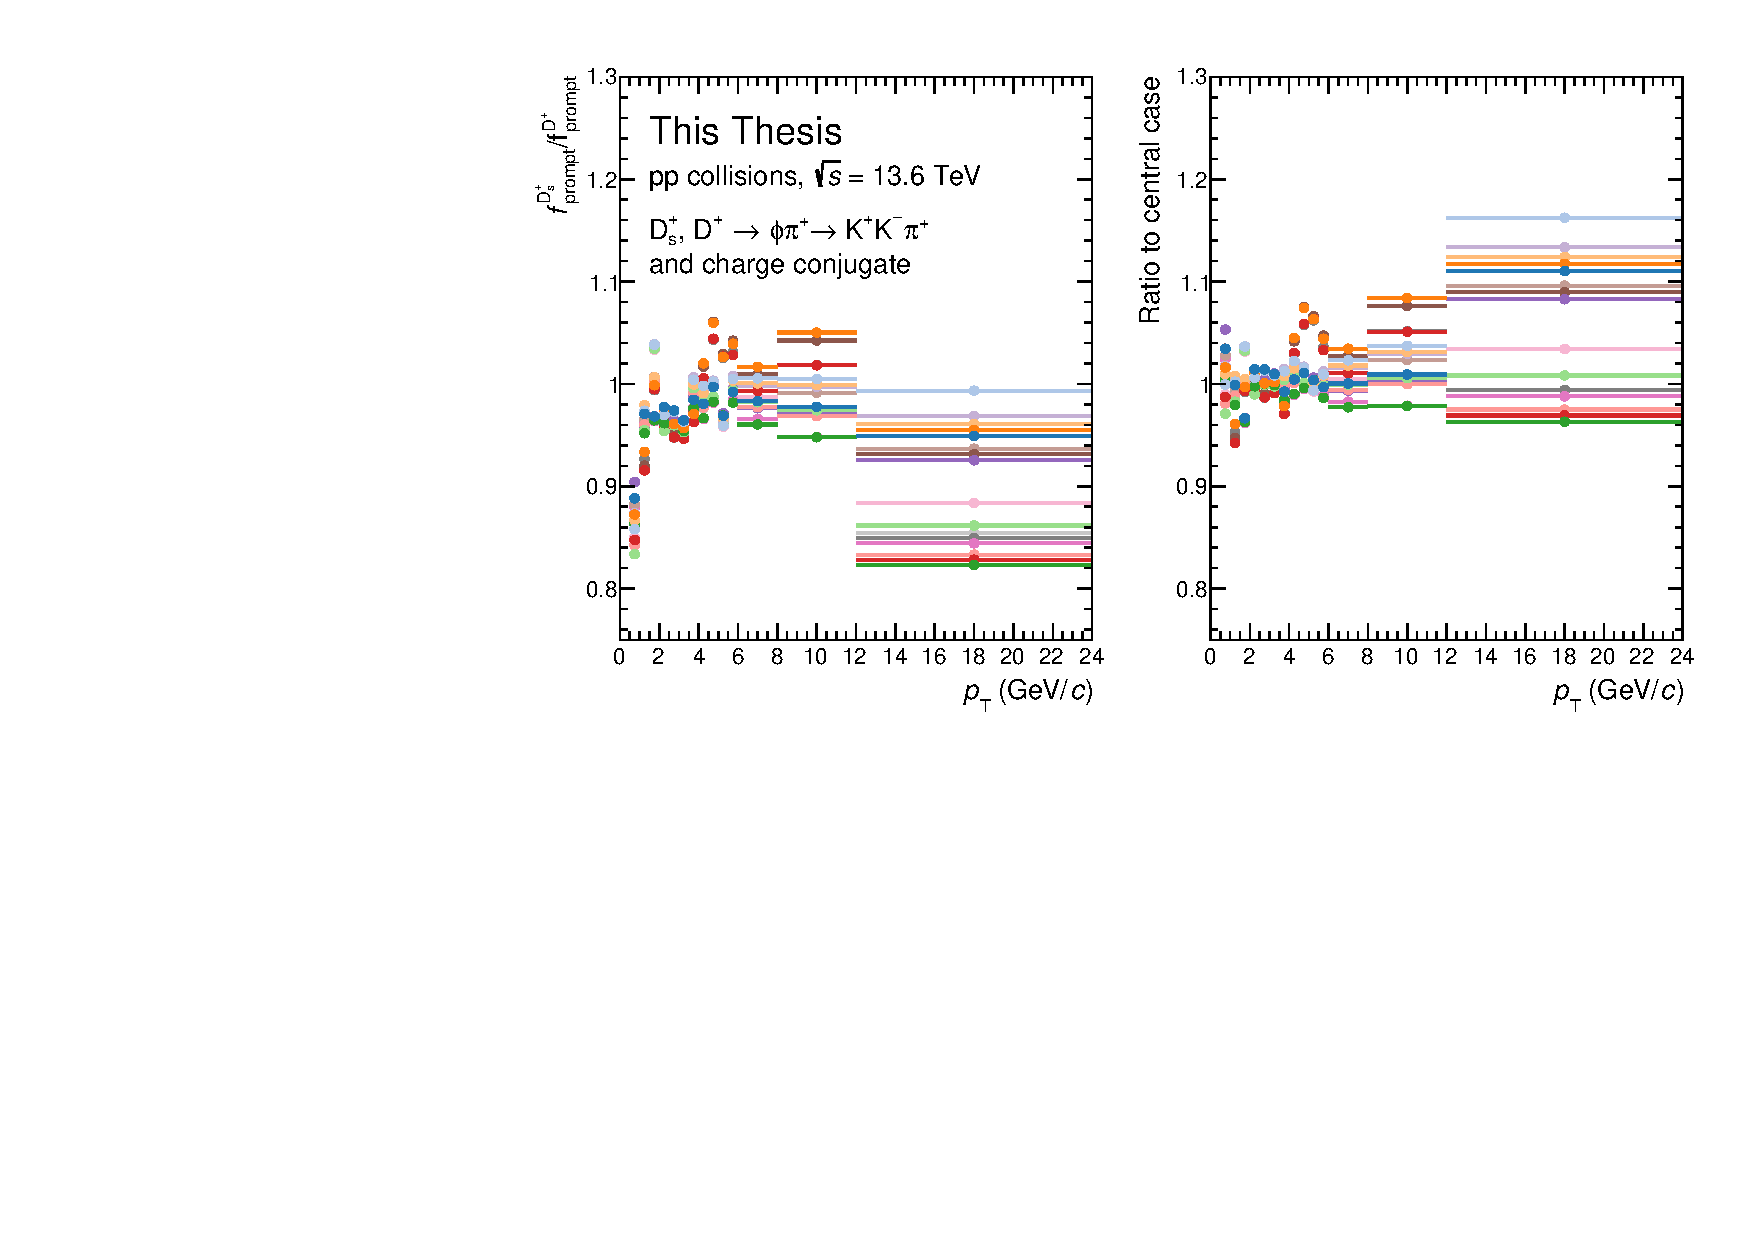
\includegraphics[width=\textwidth]{Figures/Chapter 6/PromptFracSyst.pdf}
    \caption{Results for the evaluation of the systematic uncertainty on the \fp correction. In the left panel, the different \fpds/\fpdpl corrections obtained with different sets of BDT selections are shown. In the right panel, their ratio to that obtained in the central case is reported.}
    \label{fig:fp_syst} 
    \end{center}
\end{figure}

\subsection{\texorpdfstring{Generated Monte Carlo \pt shape}{Generated Monte Carlo pT shape}}
A non-realistic \pt shape of the generated D mesons in the MC simulations could lead to a bias in the determination of the efficiency because of the \pt dependence of the \aeff corrections within the \pt intervals considered in the analysis. This source of systematic uncertainty is expected to be negligible, as: i) it was observed to have almost no impact for D mesons in previous analyses (e.g., in Refs.~\cite{ALICE:2021mgk} and~\cite{ALICE:2023sgl}), ii) because possible biases in the \pt shape of the generated D mesons would affect both \ds and \dpl mesons in a similar way, canceling out in the ratio, and iii) because very narrow \pt intervals are considered in the analysis. Nonetheless, the efficiency steeply increases with increasing \pt at low \pt, as shown in Fig.~\ref{fig:Aeff}. Therefore, it was checked that changes in the \pt distribution of generated D mesons in the MC simulations do not affect the results. The systematic uncertainty is estimated by changing the \pt distribution of the generated D mesons in the MC simulations used for the evaluation of the \aeff corrections, which are based on the \textsc{Pythia~8}~\cite{Bierlich:2022pfr} with colour-reconnection Mode~2~\cite{Christiansen:2015yqa} event generator, as described in Sec.~\ref{sec:aeff}. The \pt distribution of the generated D mesons is modified to that predicted by FONLL~\cite{Cacciari:1998it}. Both \textsc{Pythia~8} with colour-reconnection Mode~2 and FONLL predictions describe the \pt-differential cross-section of D mesons measured by the ALICE Collaboration in pp collisions at $\sqs=13$~\tev~\cite{ALICE:2021mgk}, and are therefore suitable models to describe the \pt shape of the D mesons.


The \pt distributions of \ds (\dpl) mesons are shown in the top-left (top-right) panel of Fig.~\ref{fig:MCptshape} for \textsc{Pythia}~8 (filled markers) and FONLL (void markers) predictions. In the bottom-left panel, the ratio between the FONLL and \textsc{Pythia} \pt distributions is shown for \ds and \dpl mesons. Lastly, the bottom-right panel shows the ratio between the FONLL- and \textsc{Pythia}~8-based \aeffpds/\aeffpdpl factors, which is the quantity that is used to correct the \ds/\dpl production yield ratio in Eq.~\ref{eq:DsDplusRatio}. The systematic uncertainty is estimated as the difference between the central result (obtained with \textsc{Pythia}~8 simulations) and the one obtained with the FONLL \pt shape. It resulted to be $<1\%$ for the considered \pt intervals, with the exception of the lowest interval, where a $1\%$ effect is present. However, given that this uncertainty is much smaller than the other sources of systematic uncertainty, it is not considered in the final result.

\begin{figure}[tb]
    \begin{center}
    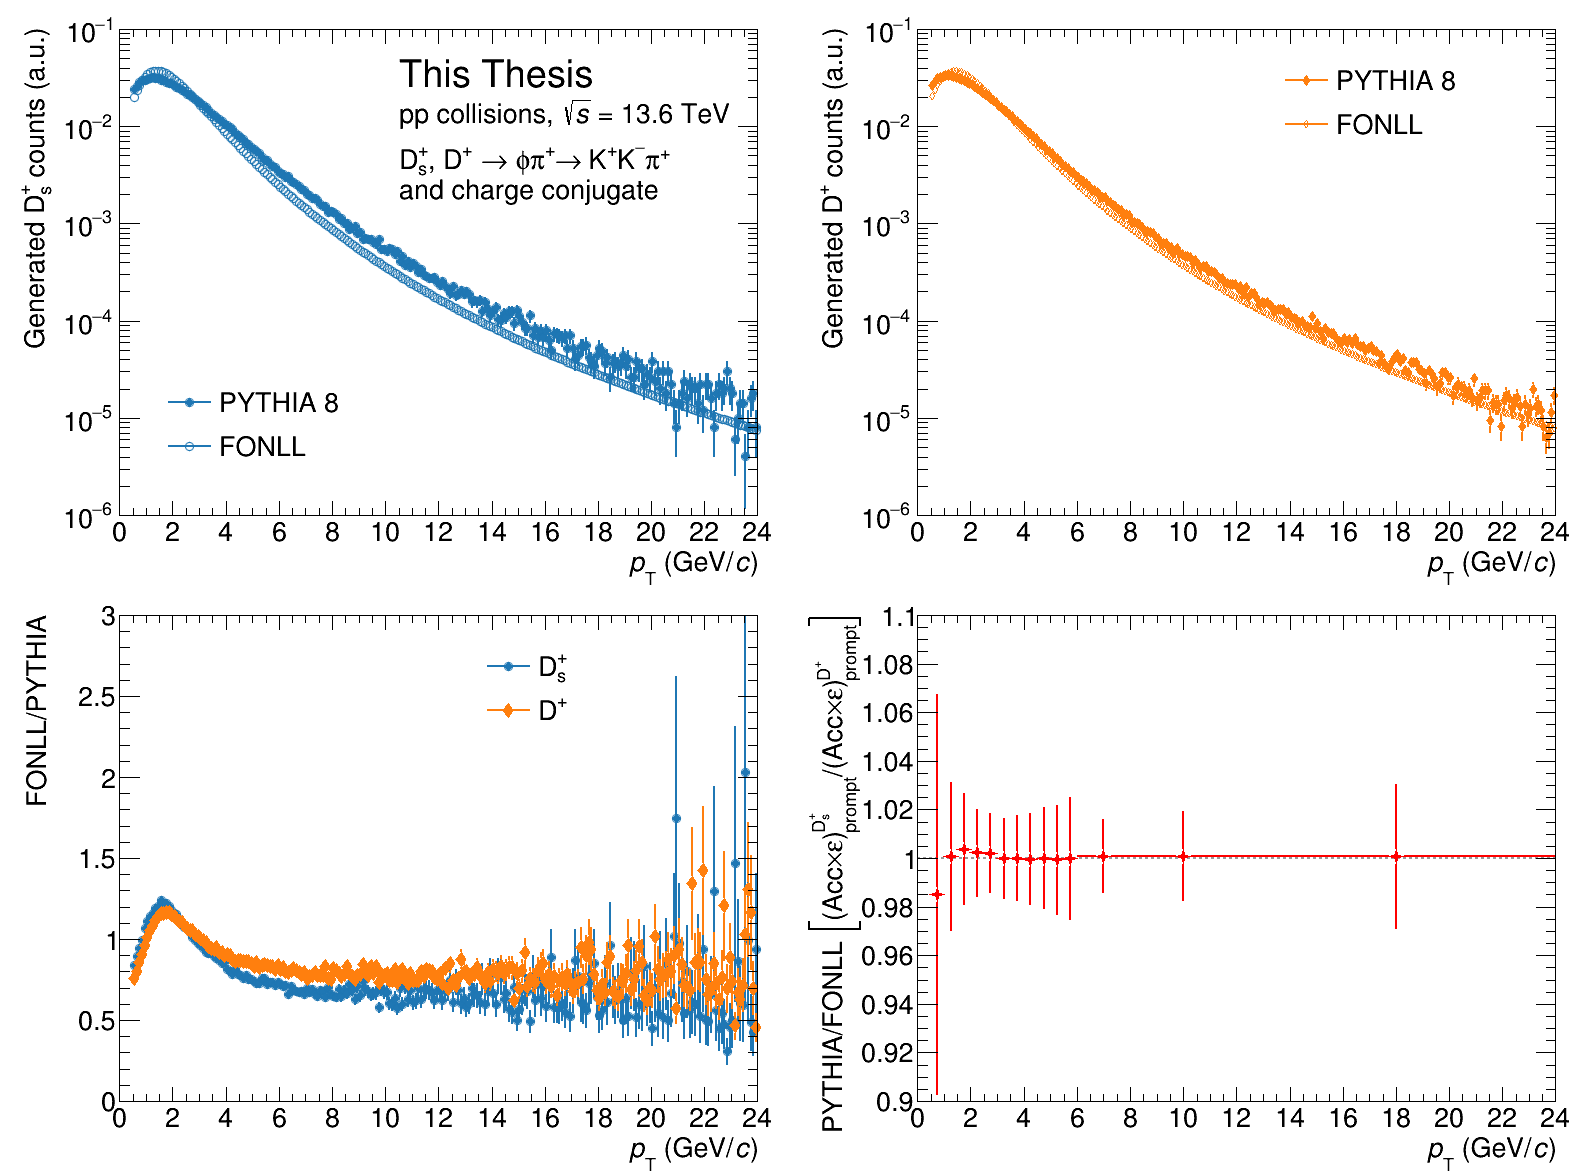
\includegraphics[width=\textwidth]{Figures/Chapter 6/PtShape.png}
    \caption{Comparison of the \pt distributions of generated \ds (left panel) and \dpl (right panel) mesons in the MC simulations used for evaluating the \aeff corrections. The distributions obtained with the \textsc{Pythia~8} event generator are shown with filled markers, while those obtained with FONLL are shown with void markers.} 
    \label{fig:MCptshape} 
    \end{center}
\end{figure}

\subsection{Summary of systematic uncertainties}
The total systematic uncertainty assigned to the different \pt intervals considered in the analysis is evaluated by summing in quadrature the contributions from the different sources of systematic uncertainty, as the sources are considered to be uncorrelated. The assigned systematic uncertainty ranges from 4\% to 13\% depending on \pt. A summary of the considered systematic uncertainties, together with the total systematic uncertainty on the \ds/\dpl production yield ratio, is reported in Table~\ref{tab:recapSyst}.

\begin{table}[htb]
    \centering
    \caption{Summary of the assigned systematic uncertainties on the \ds/\dpl production yield ratio.}
    \label{tab:recapSyst}
    \vspace*{0.3cm}
    \resizebox{\columnwidth}{!}{%
    \begin{tabular}{c|cccc|c|c}
    \toprule
    \multirow{2}{*}{\pt (\gevc)} & Raw yield  & BDT selection  & Tracking & Prompt  & Tot. syst. & BR \\
    & extraction (\%) & efficiency (\%) & performance (\%) & fraction (\%)& unc. (\%) & (\%)\\
    \midrule
    0.5$-$1 & 3     & 10    & 8     & 2     & 13    & \multirow{14}{*}{$^{+3.7}_{-4.0}$} \\
    1$-$1.5 & 3     & 5     & 2     & 2     & 7     & \\
    1.5$-$2 & 3     & 3     & 2     & 2     & 5     & \\
    2$-$2.5 & 3     & 3     & 2     & 1     & 5     & \\
    2.5$-$3 & 3     & 2     & 2     & 1     & 4     & \\
    3$-$3.5 & 3     & 2     & 1     & 1     & 4     & \\
    3.5$-$4 & 3     & 1     & 1     & 1     & 4     & \\
    4$-$4.5 & 5     & 1     & 1     & 2     & 6     & \\
    4.5$-$5 & 5     & 1     & 1     & 2     & 6     & \\
    5$-$5.5 & 5     & 2     & 1     & 2     & 6     & \\
    5.5$-$6 & 5     & 2     & 1     & 2     & 6     & \\
    6$-$8   & 8     & 2     & 1     & 2     & 8     & \\
    8$-$12  & 9     & 2     & 1     & 3     & 10    & \\
    12$-$24 & 10    & 2     & 2     & 4     & 13    & \\
    \bottomrule
    \end{tabular}%
    }
\end{table}
  